\begin{figure}[H]
\centering
\newcommand{\wagd}{\columnwidth+1.3cm}  % width airline decomp
\newcommand{\hagd}{3.5cm}  % height airline decomp
\newcommand{\mb}{\hspace{-0.8cm}}  % move back
%\newcommand{\ard}{../figures/decomposition/11-Feb-01-airline-s}  % airline results dir
\newcommand{\ard}{../figures/decomposition/31-Jan-v301-airline-months}  % airline results dir
\begin{tabular}{c}
\mb 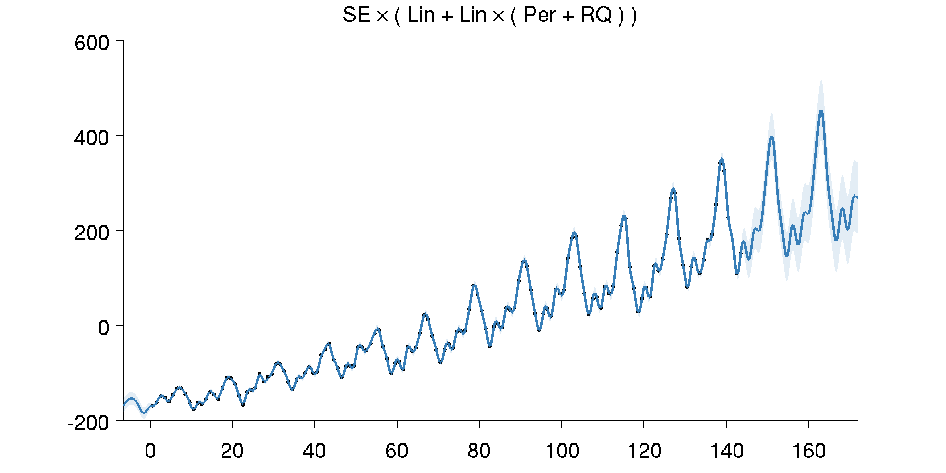
\includegraphics[width=\wagd,height=\hagd]{\ard/01-airline-months_all} \\
 = \\ 
\mb 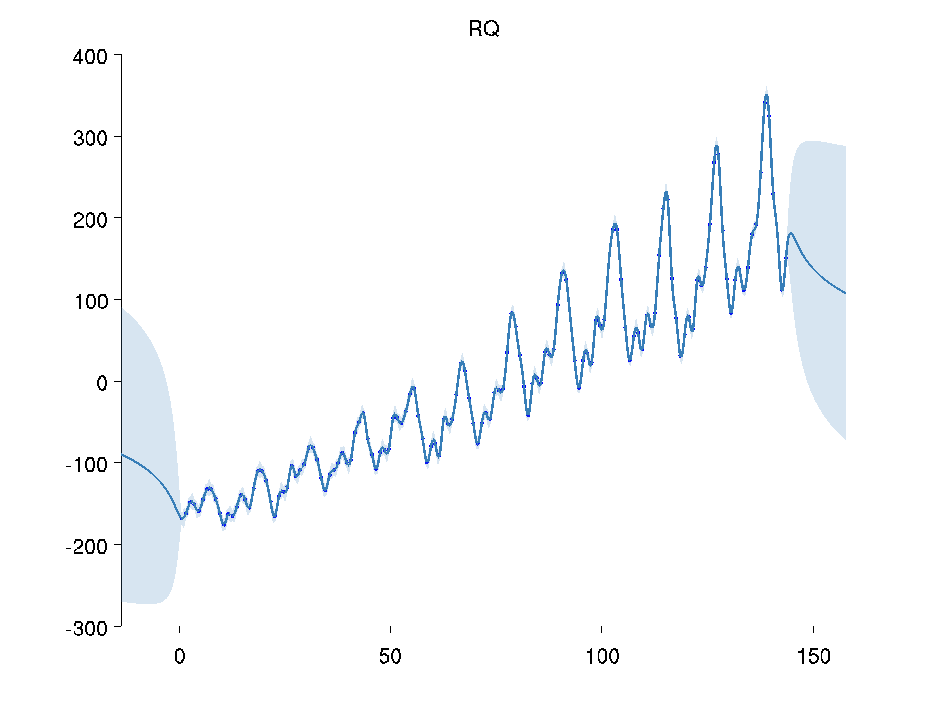
\includegraphics[width=\wagd,height=\hagd]{\ard/01-airline-months_1} \\
 + \\
\mb 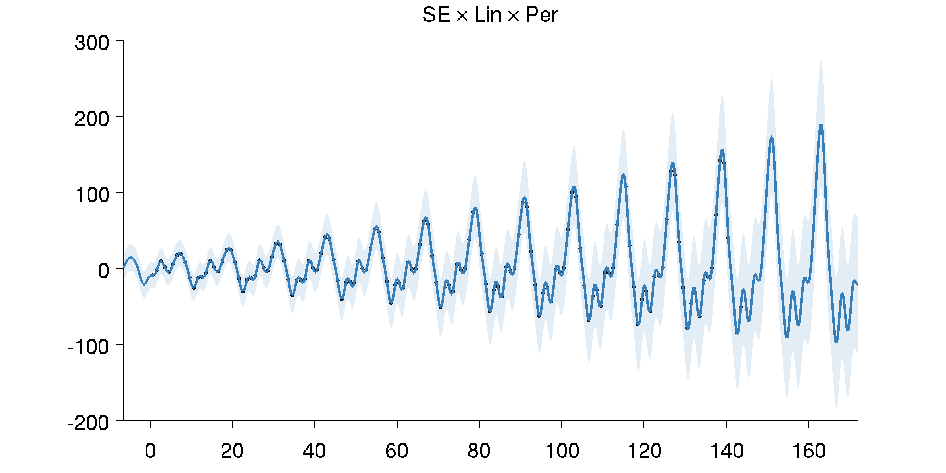
\includegraphics[width=\wagd,height=\hagd]{\ard/01-airline-months_2} \\
 + \\
\mb 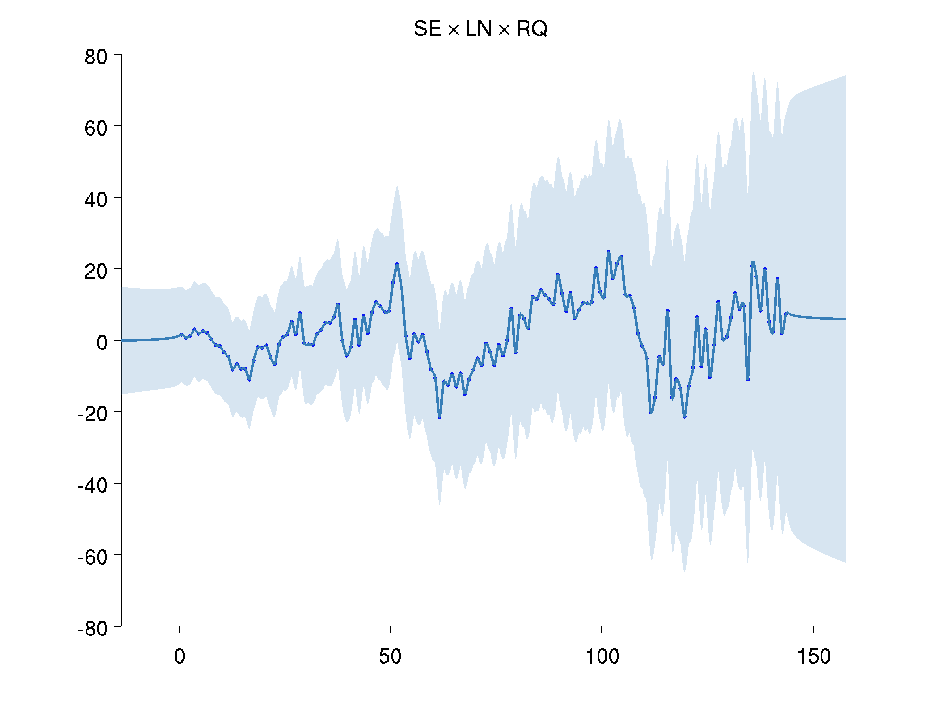
\includegraphics[width=\wagd,height=\hagd]{\ard/01-airline-months_3} \\
 + \\
\mb 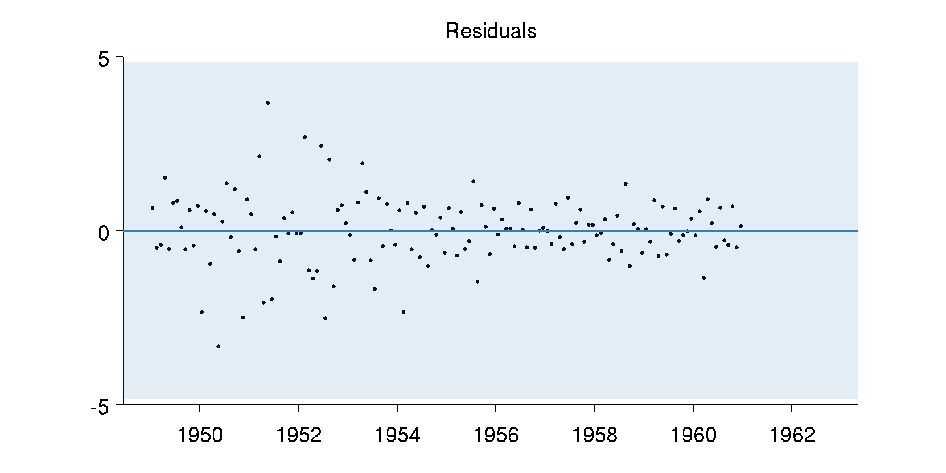
\includegraphics[width=\wagd,height=\hagd]{\ard/01-airline-months_resid}
\end{tabular}
\caption{First row:  The airline dataset and posterior after a search of depth 10.  Subsequent rows: Additive decomposition of posterior into long-term smooth trend, yearly variation, and short-term deviations.  Due to the linear kernel, the marginal variance grows over time, making this a heteroskedastic model. 
%\TBD{RBG: We allow heteroskedastic noise in our models?}
}
\label{fig:airline_decomp}
\end{figure}
